% !TeX program = lualatex
\documentclass[9pt,aspectratio=169]{beamer}
\graphicspath{{img/}{./}}
%\usepackage[spanish]{babel} % Uncomment to change language
\usepackage{tikz}
\usepackage{booktabs}
\usepackage{csquotes}
\usepackage[backend=biber, style=authoryear]{biblatex}
    \addbibresource{biblio.bib}
    \renewcommand*{\bibfont}{\scriptsize} % Change bibliography text size
    \AtEveryBibitem{\clearfield{title}}
\usepackage[table,xcdraw]{xcolor}
\usepackage{colortbl}
\usepackage{caption}
\usepackage{multicol}
\usepackage{dirtytalk}
\usepackage[shortlabels]{enumitem}
\usepackage[version=4]{mhchem}
\usepackage{colortbl}

% --------------------------------------
% Add 'Journal' field to the citations
% --------------------------------------
\renewbibmacro*{cite}{%
  % If there is no shorthand field
  \iffieldundef{shorthand}
    {%
      % Check if both labelname and labelyear are undefined
      \ifthenelse{\ifnameundef{labelname}\OR\iffieldundef{labelyear}}
        {%
          % If both are undefined, use the label macro
          \usebibmacro{cite:label}%
          \setunit{\printdelim{nonameyeardelim}}%
        }
        {%
          % Otherwise, print the author name(s)
          \printnames{labelname}%
          \setunit{\printdelim{nameyeardelim}}%
        }%
      % Always print the year (labeldate and extradate)
      \usebibmacro{cite:labeldate+extradate}%
      % Add a comma and space after the year
      \setunit{\addcomma\space}%
      % Print the journal information
      \usebibmacro{journal}%
    }
    {%
      % If shorthand is defined, use the shorthand macro
      \usebibmacro{cite:shorthand}%
    }%
}

% ------------------------------
% BEAMER CONFIG
% ------------------------------
\usefonttheme{structurebold} % Titles as bold
\useinnertheme{rectangles} % Outline bulletpoints as circles
\setbeamertemplate{caption}[numbered] % Numbered in captions
\captionsetup{font=scriptsize, justification=centering} % Caption text size

% Fonts ----
% Custom fonts: https://www.overleaf.com/learn/latex/Questions/I_have_a_custom_font_I%27d_like_to_load_to_my_document._How_can_I_do_this%3F#Using_custom_fonts_with_XeLaTeX_and_LuaLaTeX
\usepackage{fontspec}
\usepackage{fontawesome}

% Set the main font family to be Serif
\usefonttheme{serif}

% Establish the font families
\setmainfont{XCharter}
\setsansfont{Cabin}

% Costumize Beamer fonts
\setbeamerfont{title}{size=\huge, series=\bfseries, family=\sffamily}
\setbeamerfont{frametitle}{series=\bfseries, family=\sffamily}
\setbeamerfont{framesubtitle}{series=\bfseries, family=\sffamily}
\setbeamerfont{subtitle}{size=\small, series=\mdseries, shape=\itshape, family=\sffamily}
\setbeamerfont{author}{size=\normalsize, series=\mdseries, family=\sffamily}
\setbeamerfont{institute}{size=\normalsize, series=\mdseries, family=\sffamily}

% Theme ----
\usetheme{Boadilla}

% Colors ----
\definecolor{primary-color}{HTML}{0B3550}
\definecolor{secondary-color}{HTML}{CF8485}
\definecolor{tertiary-color}{HTML}{4E83A4}
\definecolor{complement-1}{HTML}{A02B93}
\definecolor{complement-2}{HTML}{4EA72E}

\definecolor{complement-text}{HTML}{545454} % #545454

\setbeamercolor{structure}{fg=primary-color}
\setbeamercolor{frametitle}{bg=primary-color,fg=white}
\setbeamersize{text margin left=1cm, text margin right=1cm}

% Title and fonts ----
\setbeamercolor{title}{fg=primary-color}
\setbeamercolor{subtitle}{fg=complement-text}


% Title card ----
\titlegraphic{
\begin{tikzpicture}[overlay,remember picture]
    \node[anchor=south, yshift=-3pt] at (current page.south){
        
\includegraphics[width=1.05\textwidth]{img/title-card.png}
    };
\end{tikzpicture}
}

% Title slides for sections ----
\AtBeginSection[]{
  \begin{frame}
    \vfill
    \centering
    \begin{beamercolorbox}[sep=8pt,center,shadow=true,rounded=true]{title}
      \usebeamerfont{title}\insertsectionhead\par%
    \end{beamercolorbox}
    \vfill
  \end{frame}
}

% Fontawesome as bulletpoints ----
\newcommand{\usageitem}[1]{
  \item[ {\makebox[2em]{\strut #1}} ]
}
\newcommand{\goal}{ \usageitem{\centering\color{secondary-color}\faBullseye} }
\newcommand{\conclusion}{ \usageitem{\centering\color{secondary-color}\faArrowCircleRight} }
\newcommand{\plus}{ \usageitem{\centering\color{secondary-color}\faPlusCircle} }

% ------------------------------
% PRESENTATION INFORMATION
% ------------------------------

% Presentation titles ----
\title[Article revision]{Article revision}
\subtitle{\textcite{ziyatdinov2023,young2022}} % can be removed/commented

% Presentation date or conference/meeting name ----
% The optional parameter can contain a shortened version to appear on 
% the bottom of every slide, while the required parameter value is output to the title slide
% -------------------------------------------------
\date[\today]{{\small}\\{\footnotesize\today}} 

% Presenter name(s) ----
% The optional parameter can contain a shortened version to appear on the bottom of every slide, while the main parameter will appear on the title slide
% ----------------------
\author[Olvera-Hernandez R.]{Roberto Olvera-Hernandez} 

% Your institution ----
% The optional parameter can be used for the institution shorthand and will appear on the bottom of every slide after author names, while the required parameter is used on the title slide and can include your email address or additional information on separate lines
% ----------------------
\institute[CCG - UNAM]{\textcolor{primary-color}{Center for Genomic Sciences (CCG),} \\ National Autonomous University of Mexico (UNAM)} 

% -----------------------
% DOCUMENT
% -----------------------
\begin{document}
{
    \setbeamertemplate{headline}{}
    % TITLE CARD ----
    \begin{frame}
        \vspace{54pt}
        \maketitle
    \end{frame}
}
\addtocounter{framenumber}{-1}

% Table of Contents ----
\begin{frame}
    \frametitle{Contents}
        \tableofcontents
\end{frame}

% ---------------------
% CONTENTS
% ---------------------

\section{Mexico City Prospective Study (MCPS)}

% ----------------------------------
% RECRUITMENT AND BASELINE DATA
% ----------------------------------
\subsection{Recruitment and baseline data}

% Overview -------------
\begin{frame}{Overview}
    \begin{columns}
        % Column with texth
        \begin{column}{0.45\textwidth}
            Over \highlight{150,000 participants} were recruited in two districts between \highlight{1998 and 2004}.
            \begin{itemize}
                \item Baseline questionnaire.
                \item Blood samples.
                \item Physical measurements.
                \item Linkage to mortality.
            \end{itemize}
            % Article title header
            \begin{figure}[htpb]
                \centering
                
\includegraphics[width=0.95\textwidth]{ziyatdinov2023/tapia-conyer2006_header.png}
            \end{figure}

        \end{column}
        % Columns with image
        \begin{column}{0.45\textwidth}
            \begin{figure}[htpb]
                \centering
                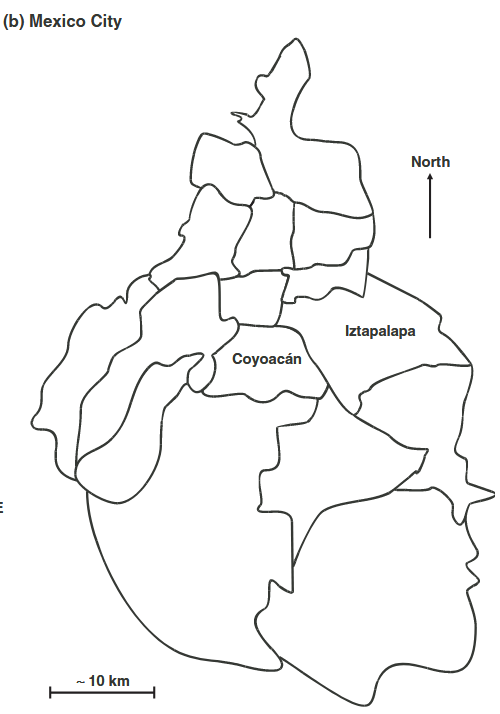
\includegraphics[width=0.45\textwidth]{ziyatdinov2023/map.png}
                \caption{Map showing the location of the MCPS districts \parencite{tapia-conyer-2006}.}
                \label{fig:mcps-main-map}
            \end{figure}
        \end{column}
    \end{columns}
\end{frame}

% Baseline data -------------
\begin{frame}{Baseline data}

    \vspace{-3mm}
    % Column A
    \begin{columns}[t]
        {\footnotesize
        \begin{column}{0.3\textwidth}

            % Socio-demographic - Textblock
            \begin{block}{Socio-demographic}<1->
                \begin{itemize}
                    \item Age and sex
                    \item Area of residence
                    \item Marital status
                    \item Educational achievement
                    \item Occupation
                    \item Income
                    \item Health service provider
                \end{itemize}
            \end{block}

            % Lifestyle - Textblock
            \begin{block}{Lifestyle characteristics}<2->
                \begin{itemize}
                    \item Diet (fruit/vegetables, fried food, types of oil)
                    \item Smoking and alcohol
                    \item Physical activity
                    \item Sleep duration
                \end{itemize}
            \end{block}

        \end{column}

        % Column B
        \begin{column}{0.3\textwidth}

            % Reproductive history - Textblock
            \begin{block}{Reproductive history (women)}<3->
                \begin{itemize}
                    \item Menopausal status
                    \item Hysteroctomy
                    \item Oopheroctomy
                    \item HRT
                    \item Contraceptive use
                    \item Pregnancy (age and number)
                \end{itemize}
            \end{block}

            % Physical measurements - Textblock
            \begin{block}{Physical measurements}<4->
                \begin{itemize}
                    \item Height
                    \item Weight
                    \item Waist and hip circumferece
                    \item Systolic and diastolic blood pressure
                \end{itemize}
            \end{block}

        \end{column}

        % Column C
        \begin{column}{0.3\textwidth}

            % Blood samples - Textblock
            \begin{block}{Blood samples}<5->
                \begin{itemize}
                    \item Plasma \& buffy coat
                    \item HbA1c and other essays
                    \item NMR metabolomics (e.g. fatty acids, cholines, lipoprotein subclasses, etc.)
                \end{itemize}
            \end{block}

            % Prior diseases and medications - Textblock
            \begin{block}{Prior diseases and medications}<6->
                Participants were asked if they had ever been diagnosed with any of the listed diseases (binary: \textit{Yes} or \textit{No}).
            \end{block}

        \end{column}
        }
    \end{columns}
\end{frame}

% ----------------------------------
% GENETIC OVERVIEW
% ----------------------------------
\subsection{Genetic overview}

% Genetic datasets ----------------
\begin{frame}{Genetic datasets}

    \begin{itemize}
        \item Genetic datasets were added later by \textcite{ziyatdinov2023}, making it one of the \highlight{largest} studies for \highlight{non-eurpean} populations.
        \item<2-> Comparison (WES and WGS) were made with other datasets: \textbf{UK Biobank}, \textbf{TOPMed}, \textbf{gnomAD}.
    \end{itemize}

    {\footnotesize
    \begin{columns}[t]

        \begin{column}{0.3\textwidth}
            \begin{block}{Genome-Wide Genotyping}<3->
                \begin{itemize}
                    \item Illumina --- GSAv2 chip array
                    \item 138,511 individuals
                \end{itemize}
            \end{block}
        \end{column}

        \begin{column}{0.3\textwidth}
            \begin{block}{Exome Sequencing (WES)}<4->
                \begin{itemize}
                    \item $n =$ 141,046 individuals
                \end{itemize}

                \textbf{Variants:}
                \begin{itemize}
                    \item \textit{Total:} 9.3 million.
                    \item \textit{Coding regions:} 4.0 million in 19,110 genes.
                    \item \textit{Unique MCPS:} 1.4 million.
                \end{itemize}

            \end{block}        
        \end{column}

        \begin{column}{0.3\textwidth}
            \begin{block}{Whole-Genome Sequencing (WGS)}<5->
                \begin{itemize}
                    \item $n =$ 9,950 individuals
                \end{itemize}

                \textbf{Variants:}
                \begin{itemize}
                    \item \textit{Total:} 131.9 million.
                    \item \textit{Coding regions:} 1.5 million.
                    \item \textit{Unique MCPS:} 31.5 million.
                \end{itemize}
            \end{block}
        \end{column}
    \end{columns}
    }

    \vfill

    \uncover<6->{
        \begin{itemize}
            \item Both \textbf{WES} and \textbf{WGS} share \alert{93.2\%} of the variants, with an increment of \alert{2.3\%} on \textbf{WGS} data.
        \end{itemize}
    }
\end{frame}

\begin{frame}{WES and WGS - Comparisons}

    \begin{itemize}
        \item Lower proportion of \highlight{singletons}, indicates \textit{extensive familial relatedness}.
        \item Increased number of \highlight{predicted loss of function (pLOF)} variants.
    \end{itemize}

    \medskip

    % Modified in Excel
    \begin{figure}[htpb]
        \centering
        % Supplementary Table 3
        \includegraphics<1>[width=0.95\textwidth]{ziyatdinov2023/table-comparison-3.png}
        % Supplementary Table 7
        \includegraphics<2>[width=0.95\textwidth]{ziyatdinov2023/table-comparison-7.png}
    \end{figure}
\end{frame}

% Family networks ----------------
\begin{frame}{Family networks}

\begin{columns}
    % Column 1
    \begin{column}{0.45\textwidth} 

       \begin{exampleblock}{Estimation}<1->
            Relatedness was estimated through \textit{identity-by-descent (IBD)} sharing.
       \end{exampleblock}

       \medskip
    
       \uncover<2->{
        About \alert{71\%} of individuals have \highlight{at least one relative} present in the MCPS dataset. 

       \begin{itemize}
           \item \textbf{Parent-Offspring (PO):} 31,597 relationships.
           \item \textbf{Sibling Pairs (FS):} 29,482 relationships.
           \item \textbf{Second Degree (2nd):} 47,080 relationships.
           \item \textbf{Third Degree (3rd):} 120,180 relationships.
       \end{itemize}
       }

    \end{column}
    % Column 2
    \begin{column}{0.45\textwidth}<3->
        \begin{figure}[htpb]
        \centering
        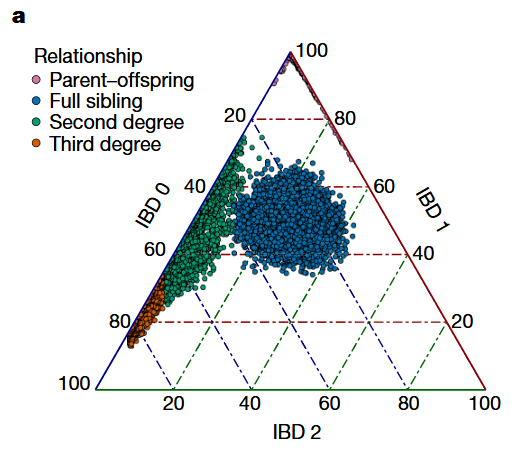
\includegraphics[width=0.95\textwidth]{ziyatdinov2023/familial-relatedness-a.png}
        \caption{Percentage of genome estimated to have zero, one or two IBD alleles \parencite{ziyatdinov2023}.}
        \label{fig:ibd-genome-percentage}
        \end{figure}
    \end{column}
\end{columns}
\end{frame}

\begin{frame}[t]{Family networks}
    \begin{figure}[htpb]
        \centering
        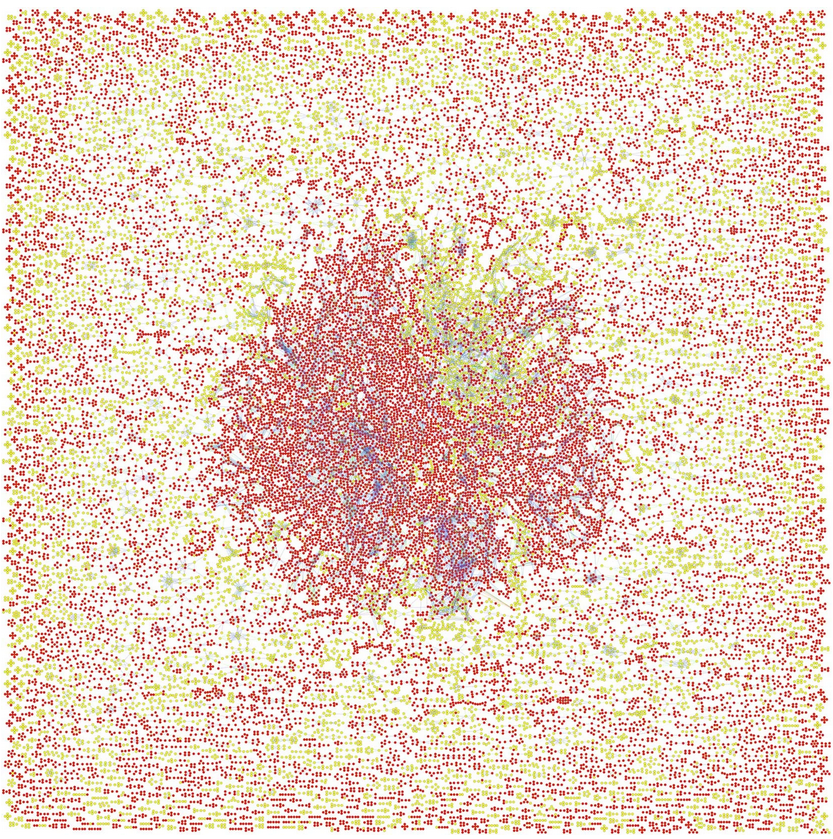
\includegraphics[height=2.25in]{ziyatdinov2023/2nd-degree-family-networks.png}
        \caption{Graph of second-degree family networks of size four or greater \parencite{ziyatdinov2023}.}
        \label{fig:2nd-degree-megaplot}
    \end{figure}
\end{frame}

\begin{frame}{Family networks}
    \begin{columns}
        % Column 1
        \begin{column}{0.5\textwidth}

            The levels of \textit{relatedness} were:
            \begin{itemize}
                \item much higher than those from the \textbf{UK Biobank (UKB)}.
                \item comparable with the \textbf{Geisinger Health Study (GHS)}--both \textbf{MCPS} and \textbf{GHS} recruited in \textit{close proximity}.
            \end{itemize}
        \end{column}

        % Image column -----
        \begin{column}{0.5\textwidth}
            \begin{figure}[htpb]
                \centering
                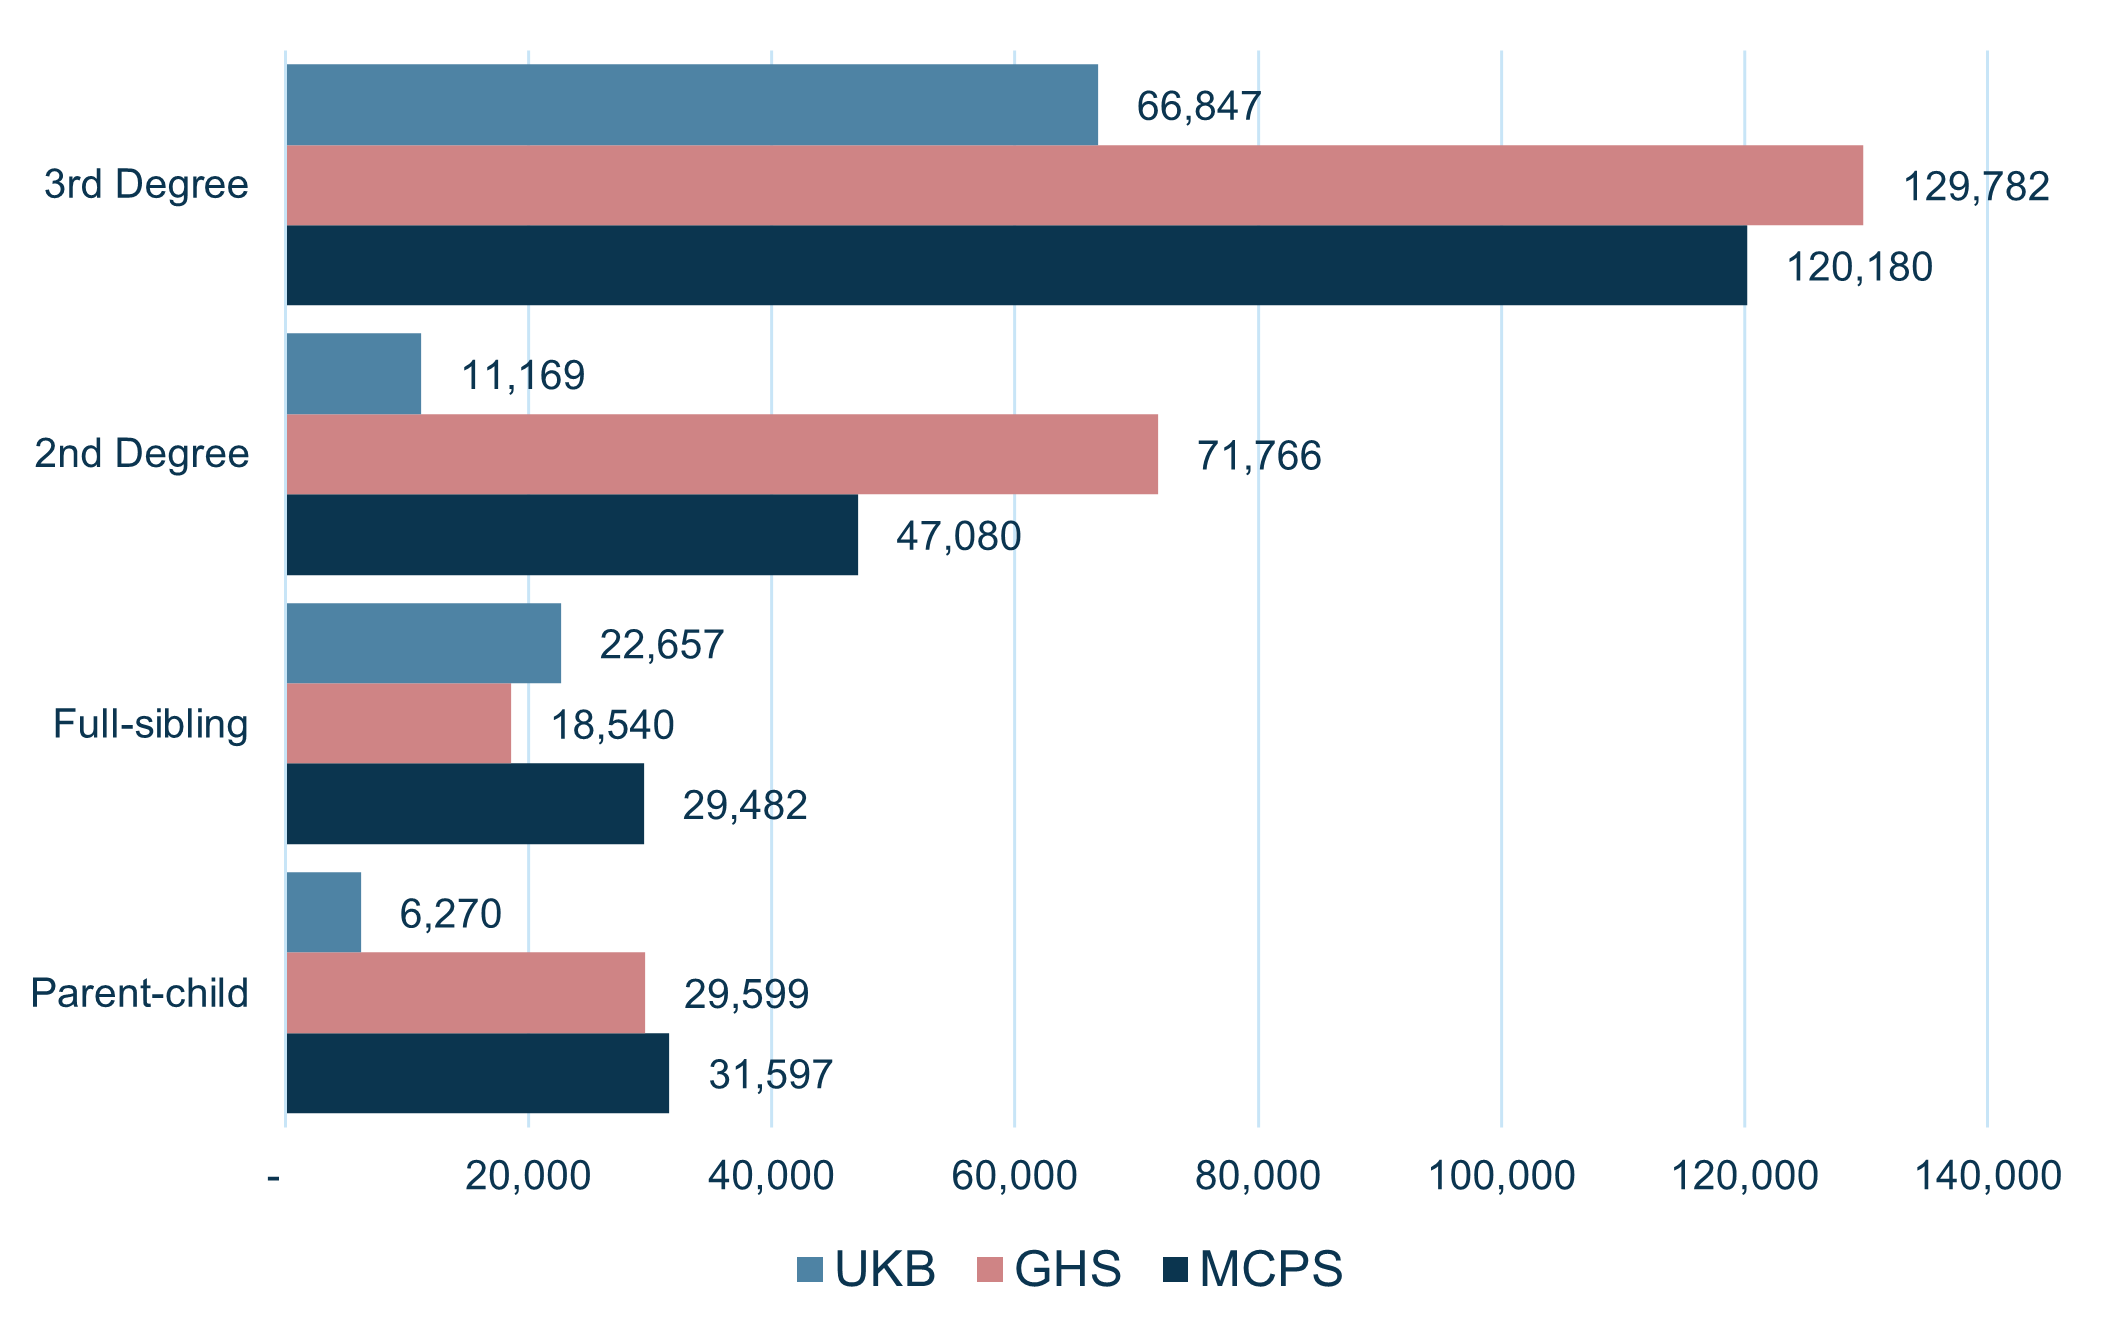
\includegraphics[width=0.95\textwidth]{ziyatdinov2023/dataset-comparison.png}
                \caption{Comparison of network sizes in MCPS, UKB and GHS. Data extracted from Supplementary Table 25 \parencite{ziyatdinov2023}.}
                \label{fig:ziyatdinov2023-nrelationships-comparison}
            \end{figure}
        \end{column}
    \end{columns}
\end{frame}

% Population structure -------------
\subsection{Population structure and ancestry}
% PCA characterization
\begin{frame}[fragile,t]{Admixture characterization (PCA)}

\begin{itemize}
    \item \textbf{1,000 Genomes Project (1KG):} 108 African (Yoruba); 107 European (Iberian).
    \item \textbf{Metabolic Analysis of an Indigenous Samples (MAIS)}\footnote{\cite{garcia-ortiz2021}}: 591 Indigenous Mexican (north, northwest, central, south, southeast).
\end{itemize}

\vfill

\begin{columns}
    \begin{column}{0.45\textwidth}
        \begin{figure}[htpb]
            \centering
            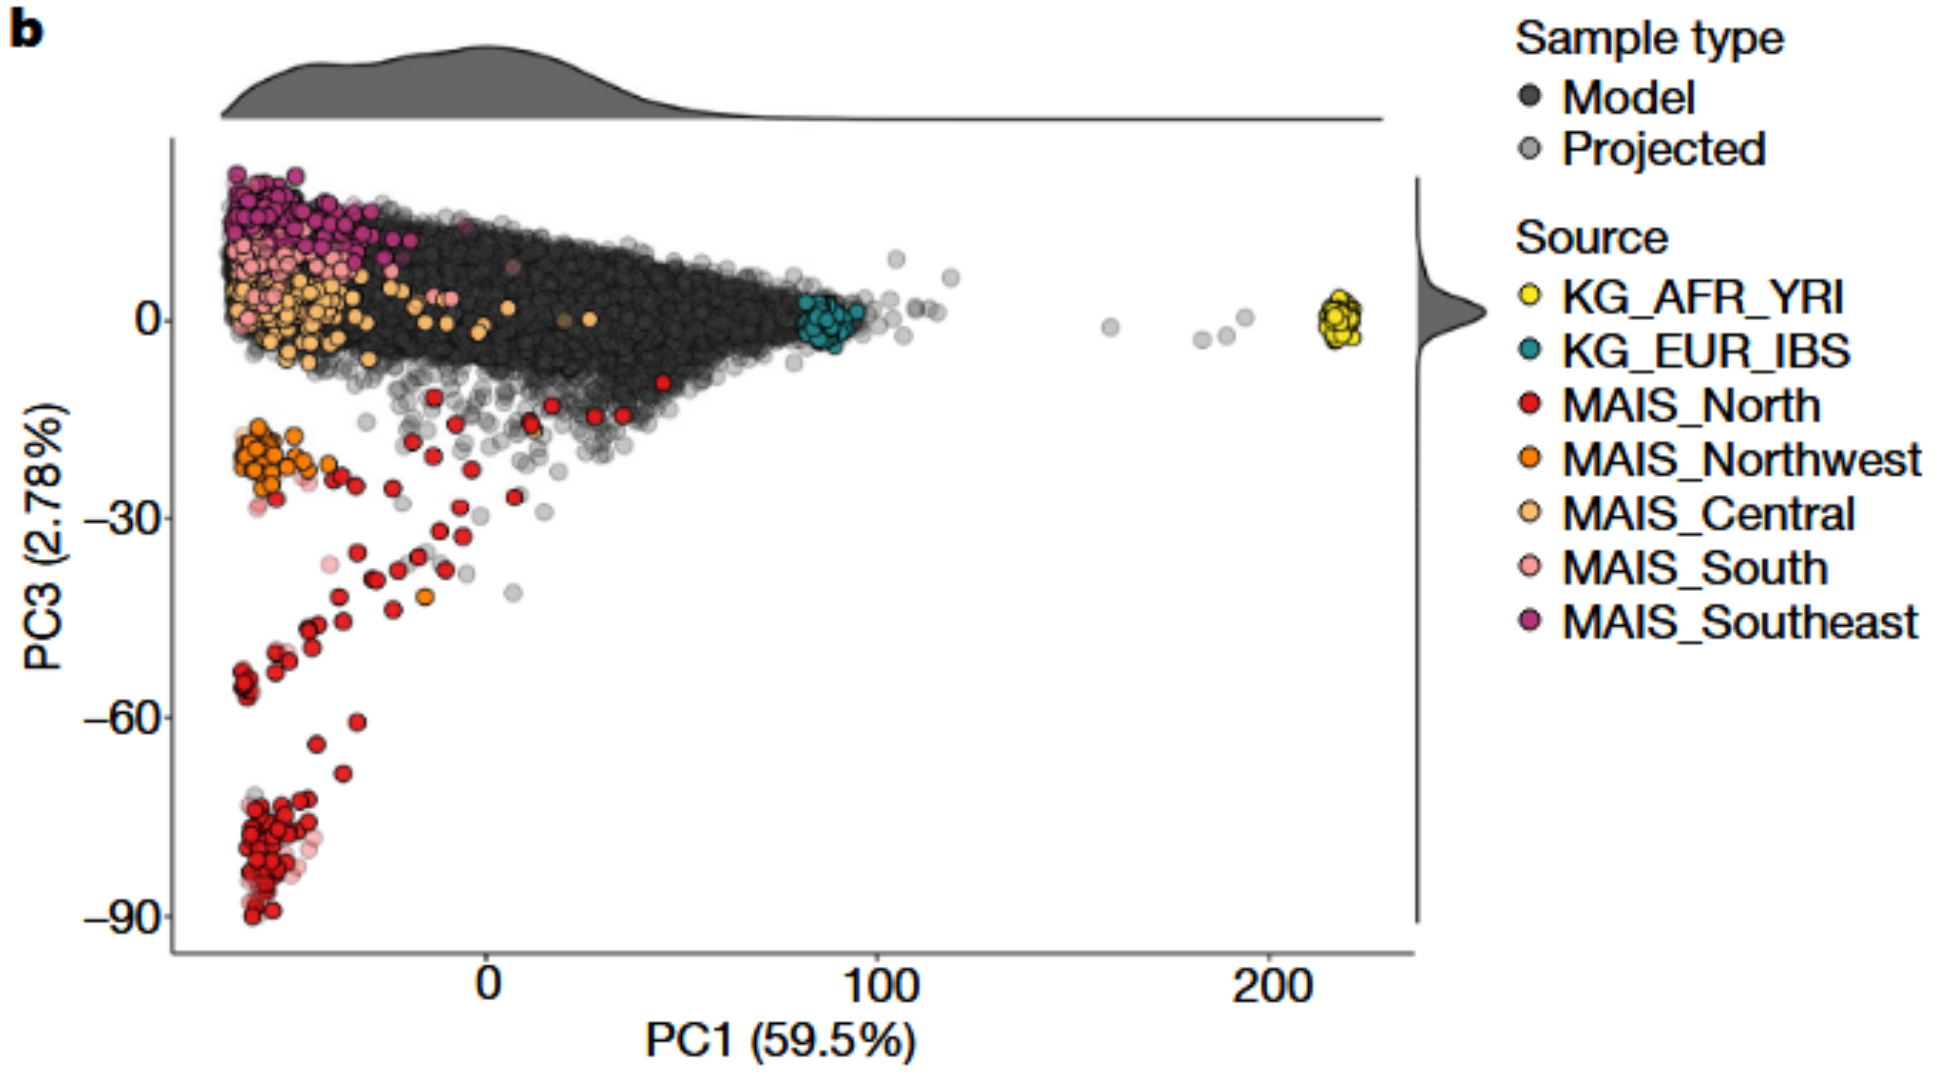
\includegraphics[width=0.95\textwidth]{ziyatdinov2023/pca-analysis-2.png}
            \caption{\textit{Model one:} projection of 500 MCPS unrelated samples \parencite{ziyatdinov2023}.}
            \label{fig:pca-1-admixture}
        \end{figure}
    \end{column}
    \begin{column}{0.45\textwidth}
        \begin{figure}[htpb]
            \centering
            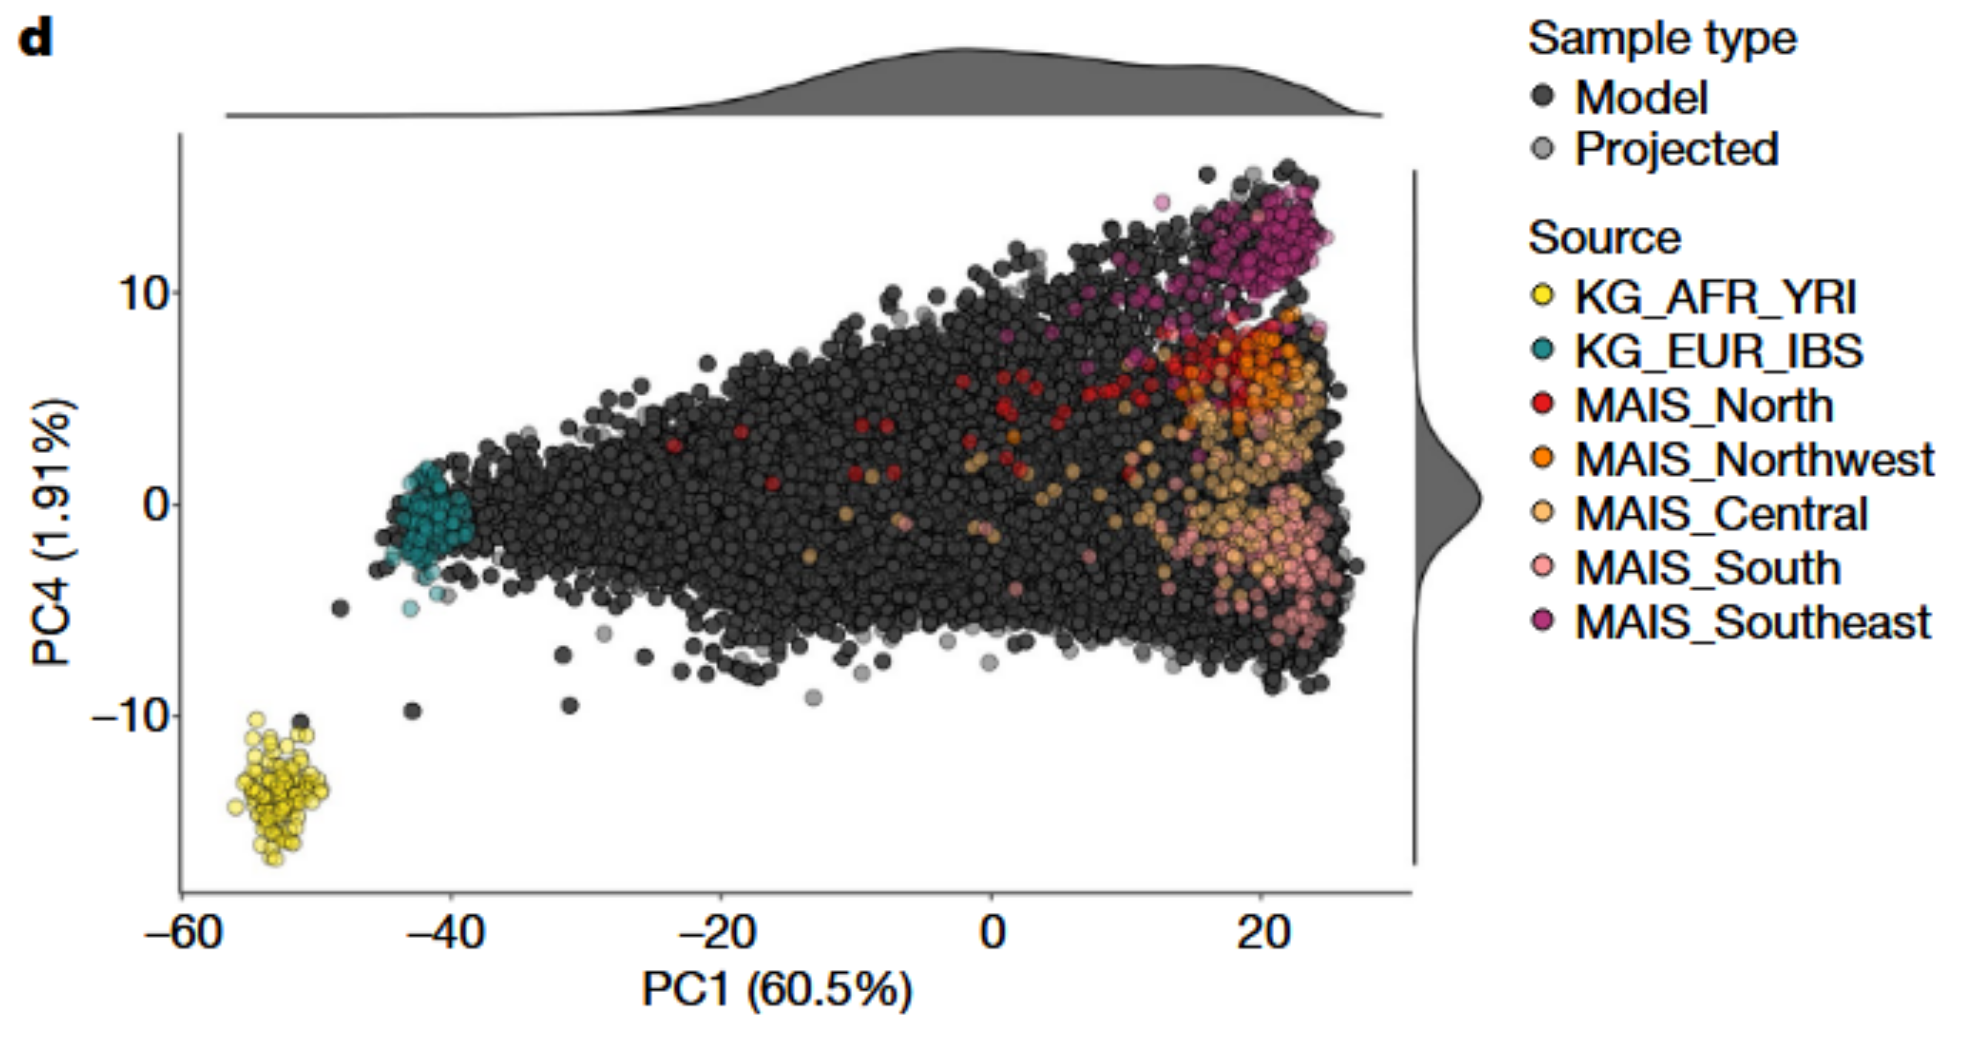
\includegraphics[width=0.95\textwidth]{ziyatdinov2023/pca-analysis-4.png}
            \caption{\textit{Model two:} projection of 58,051 MCPS unrelated samples \parencite{ziyatdinov2023}.}
            \label{fig:pca-2-admixture}
        \end{figure}
    \end{column}
\end{columns}
\end{frame}

% ADMIXTURE discrete characterization
\begin{frame}[fragile]{Discrete admixture characterization}
    \begin{figure}[htpb]
        \centering
        \includegraphics<1>[width=0.95\textwidth]{ziyatdinov2023/discrete-admixture-1.png}
        \includegraphics<2>[width=0.95\textwidth]{ziyatdinov2023/discrete-admixture-2.png}
        \includegraphics<3>[width=0.95\textwidth]{ziyatdinov2023/discrete-admixture-3.png}
        \caption{Ancestry proportion estimates for 137,511 MCPS samples. Datasets: 1KG, HGDP, and MAIS datasets are shown \parencite{ziyatdinov2023}.}
        \label{fig:discrete-admixture}
    \end{figure}
\end{frame}
%\section{Mendelian Imputation}

\subsection{Family Genome-Wide Association Studies (FGWAS)}

\begin{frame}{Why use them?}
    \begin{columns}
        % Column 1: Image
        \begin{column}{0.45\textwidth}
            \begin{figure}
                \centering
                \includegraphics[width=0.95\linewidth]{example-image-a}
                \caption{Signals captured by FGWAS in families \parencite{young2019}.}
                \label{fig:fgwas-genetic-signals}
            \end{figure}
        \end{column}

        % Column 2: Text
        \begin{column}{0.45\textwidth}
            % Block 1: 
            \begin{exampleblock}{Unbiased GWAS}<2->
                \begin{itemize}
                    \item<2-> Can discriminate \textbf{DGEs}\footnote{Direct Genetic Effects} and \textbf{Population Effects} using \textbf{parental genotypes} as controls.
                    \item<3-> Source of genetic variation is \textbf{\textit{within-family}}.
                \end{itemize}
            \end{exampleblock}

            % Block 2
            \begin{alertblock}{We lose power}<4->
                \begin{itemize}
                    \item<4-> We need \textbf{more individuals $n$} to be genotyped.
                    \item<5-> Complete parent-offspring trios are \textit{rare} in cohorts.
                \end{itemize} 
            \end{alertblock}
        \end{column}
    \end{columns}
\end{frame}

\begin{frame}[t]{Traditional GWAS Linear Model}

\only<1>{
    {\Huge
       \begin{align*}
           	\textcolor{black}{\tilde{y}_i} = 
           	\textcolor{black}{\sum_{k=1}^{K} \delta_k x_{ik}} + 
           	\textcolor{black}{z_{i}^{\prime}\gamma} +
           	\textcolor{black}{\epsilon_i}
       \end{align*} 
    }
}
\uncover<2->{
    {\Huge
       \begin{align*}
           \textcolor{azure!80!black}{\tilde{y}_i} = 
           \textcolor{green!80!black}{\sum_{k=1}^{K} \delta_k x_{ik}} + 
           \textcolor{orange!80!black}{z_{i}^{\prime}\gamma} +
           \textcolor{red!80!black}{\epsilon_i}
       \end{align*} 
    }
}

\begin{enumerate}
    \item<2-> \textbf{\color{azure!80!black} Observed fenotype} for $i$ individual
    \item<3-> \textbf{\color{green!80!black} Causal genetic component} for $x$ genotype at SNP $k$, accounts for DGE ($\delta$).
    \item<4-> \textbf{\color{orange!80!black} Confounding Effects}.
    \item<5-> \textbf{\color{red!80!black} Error}.
\end{enumerate}
   
\end{frame}

% snipar - parental imputation
\begin{frame}[fragile]{Parental genotype imputation (\textit{snipar})}

  \begin{columns}
    % Column 2: Complete data
    \begin{column}{0.30\textwidth}
      \begin{center}
        {\bfseries\color{ccgblue} Complete data}
        \includegraphics[width=0.95\textwidth]{example-image-a}
      \end{center}
    \end{column}

    % Column 2: Siblings only
    \begin{column}{0.30\textwidth}
      \begin{center}
        {\bfseries\color{ccgblue} Siblings only}
        \includegraphics[width=0.95\textwidth]{example-image-b}
      \end{center}
    \end{column}

    % Column 3: Parent-offspring
    \begin{column}{0.30\textwidth}
      \begin{center}
        {\bfseries\color{ccgblue} Parent-offspring}
        \includegraphics[width=0.95\textwidth]{example-image-c}
      \end{center}
    \end{column}

  \end{columns}

  \vfill

  \begin{center}
    GitHub (\textit{snipar}): \url{https://github.com/AlexTISYoung/snipar}
  \end{center}

\end{frame}
























% ---------------------
% BIBLIOGRAPHY
% ---------------------
\begin{frame}
    \frametitle{References}
    \begin{multicols}{2}
        \printbibliography[]
    \end{multicols}
\end{frame}

\end{document}